% !TeX root = ../analysisnote.tex

\section{Analysis method}
In this section, event plane reconstruction would be described firstly.
Second part is identification for measured particles, including identified particles($pi+$ and $pi-$), 
and weak decay particles($K_0^S$ and $\Lambda$). Last one is efficiency correction, 
including TPC tracking efficiency, TOF matching efficiency and particle reconstruction efficiency.


\subsection{Event plane reconstruction}
Event plane method is one of common method in the anisotropic flow analysis, which could be used to estimate
the reaction plane in the Heavy Ion Collision.\cite{PhysRevC.83.044913} In this analysis, we used STAR detector 
Event Plane Detector(EPD), incorporating with Time Projection Chamber to reconstructe Event Plane(EP), 
where EPD is an upgrade detector in the STAR Beam Energy Scan phase II.\cite{ADAMS2020163970} There are 12 supersectors
on EPD. And 31 tiles on each supersector are connected via optical fiber bundles.
The tile performance would be affected by its own quality and the signal intensity it received.
So the correction for each tile is necessary, which would be introduced as follow.

Recentering and shifting method are two methods which we applied to correct the raw event plane
distribution. EPD is divided to four ring groups to facilitate EP reconstruction. There are 16 rings/rows
on EPD. It is divided equally to four groups, each group have four rings. Fig.~\ref{fig:EPDgroup} show
\begin{figure}[hbt!]
\centering
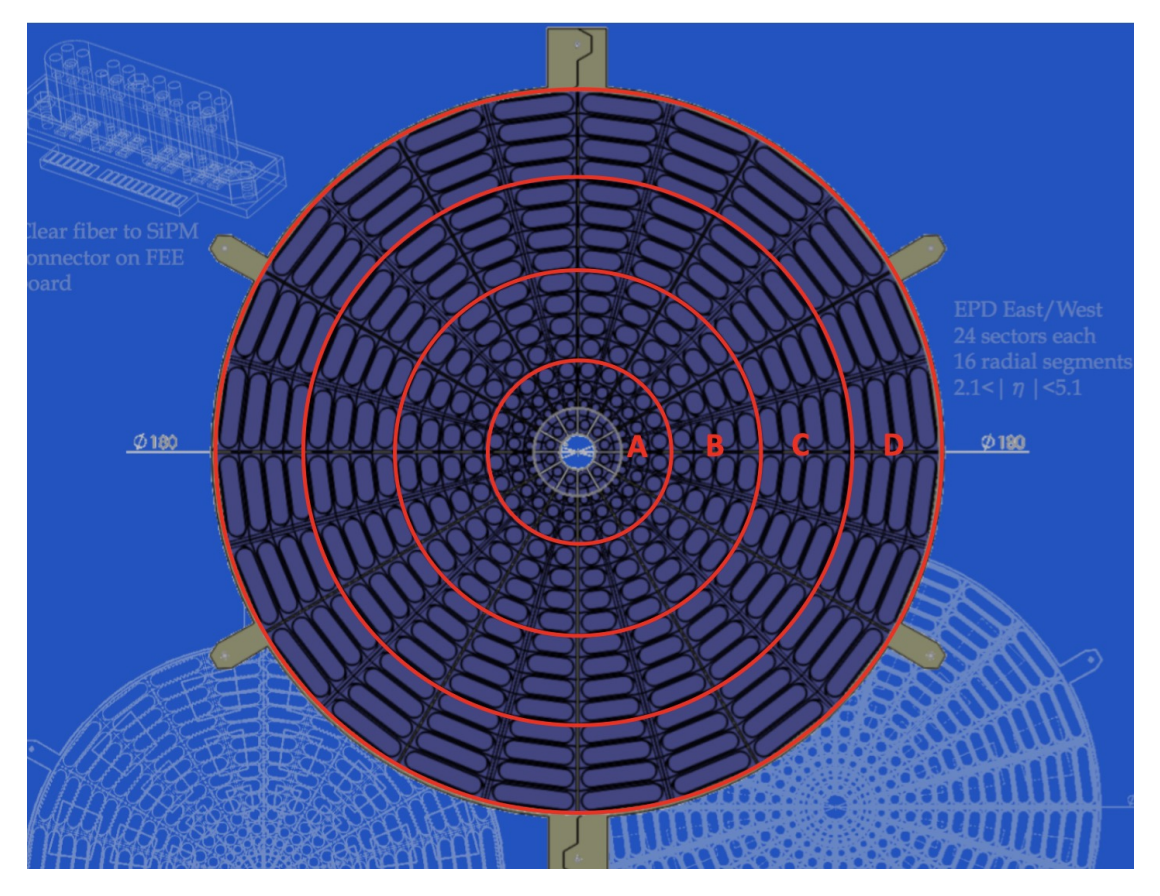
\includegraphics[width=0.45\linewidth]{figures/chapter02/EPDgroup.png}
\caption{The sketch of EPD groups.}
\label{fig:EPDgroup}
\end{figure}
groups at EPD, named as A, B, C and D. The best EP should be the one in the forward eta range, where directed flow
signal is greater than the one in middle eta range. \href{https://drupal.star.bnl.gov/STAR/system/files/FXT3gev_note_v4.pdf}{Analysis note} of one STAR published paper have approved it. 
We followed and chose EPD group A and B as target event plane in our analysis.
In this way, we can get the largest resolution applied to our analysis according to equation~\ref{eq:res_simp}
\begin{equation}
    R_n \propto v_n \sqrt{M}
\label{eq:res_simp}
\end{equation}

\subsubsection{Recentering correction}
The recentering calibration is applied to the flow vector($\vec{Q}$), which could be decomposed into 
two components, as shown by equation~\ref{eq:Qvector}, where $w_i$ is EPD tile weight, using the
calibrated value nMip(also known as ADC) based on the particle energy loss on each EPD tile, as shown by equation~\ref{eq:tile_weight}
\begin{equation}
    \overrightarrow{\mathrm{Q}}=\left(\begin{array}{l}
    Q_y \\
    Q_x
    \end{array}\right)=\left(\begin{array}{c}
    \sum_i w_i \sin (\phi_i) \\
    \sum_i w_i \cos (\phi_i)
    \end{array}\right)
\label{eq:Qvector}
\end{equation}

\begin{equation}
    w(\text { tile })= \begin{cases}0 & \text { if } n M I P<\operatorname{threshold}(0.3) \\ \text { MAX } & \text { if nMIP }>\operatorname{MAX}(2) \\ n M I P & \text { otherwise }\end{cases}
\label{eq:tile_weight}
\end{equation}
And the first order event plane angle could be obtained by equation~\ref{eq:EPangle}, where $\phi_i$ is emitted particle angle 
with respect to the laboratory system, sums goes over all hits from one event.
\begin{equation}
    \Psi_1=\tan ^{-1} \frac{\sum_i w_i \sin \left(\phi_i\right)}{\sum_i w_i \cos \left(\phi_i\right)}
\label{eq:EPangle}
\end{equation}

The recentering method is applied to the flow vertex $\vec{Q}$, so it's event by event calibration,
Which is expressed by equation~\ref{eq:recenter_method}. The angle brackets denote averaging over all events
in the same centrality and run ID.
\begin{equation}
    \vec{Q}_{r c}=\left(\begin{array}{l}
    \vec{Q}_y-\left\langle\vec{Q}_y\right\rangle \\
    \vec{Q}_x-\left\langle\vec{Q}_x\right\rangle
    \end{array}\right)
\label{eq:recenter_method}
\end{equation}

\subsubsection{Shifting correction}
The shifting calibration is a mathematical method to correct the EP distribution after recentering calibration,
which is based on Fourier transformation. In this analysis, a 20th order equation~\ref{eq:shift_method} was implemented to the event plane distribution
after recentering calibration.
\begin{equation}
\Psi_{1, \text { shift }}=\sum_i^N \frac{2}{i}\left[-\left\langle\sin \left(i \Psi_{1, r c}\right)\right\rangle \cos \left(i \Psi_{1, r c}\right)+\left\langle\cos \left(i \Psi_{1, r c}\right)\right\rangle \sin \left(i \Psi_{1, r c}\right)\right]
\label{eq:shift_method}
\end{equation}

The angle brackets in the equation denote averaging over all events in the same centrality and run ID.
And the final EP angle after recentering and shifting calibration could be obtained by equation~\ref{eq:psi_final}
\begin{equation}
\Psi_1=\Psi_{1, r c}+\Psi_{1, s h i f t}
\label{eq:psi_final}
\end{equation}

Fig.~\ref{fig:EP_distribution} show event plane distribution at 3, 3.2, 3.5 and 3.9 GeV based on all EPD rings,
where the black line show the raw distribution without any calibration, the blue line represents the EP after recentering calibration, 
and red line denote the event plane angle distribution after recentering and shifting calibration, which is "flat".
\begin{figure}[hbt!]
\centering
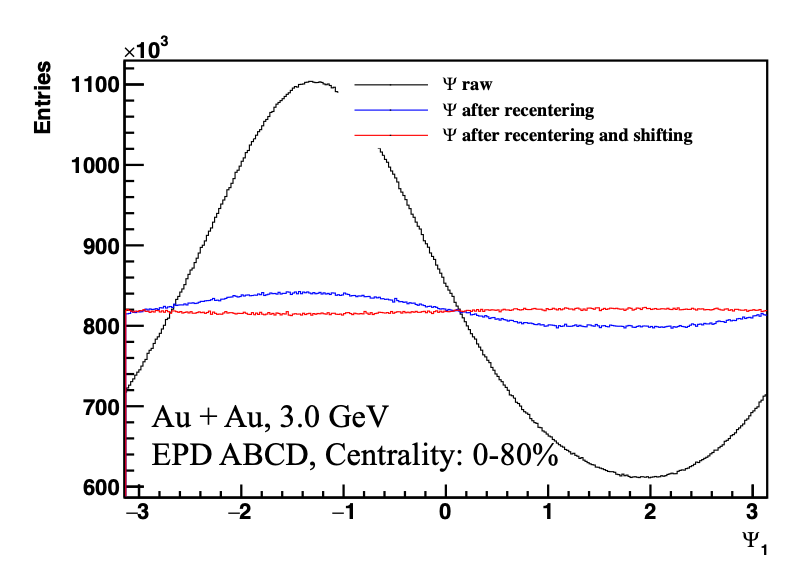
\includegraphics[width=0.45\linewidth]{figures/chapter02/EP_3GeV.png}
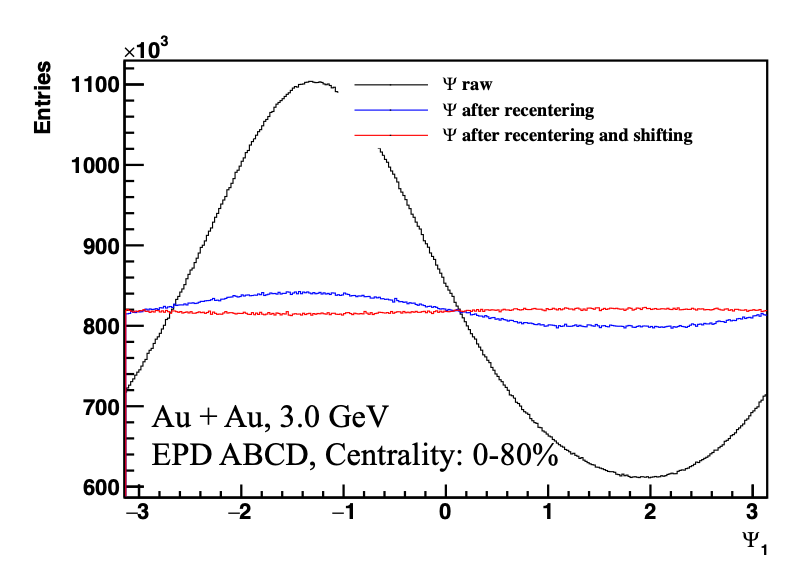
\includegraphics[width=0.45\linewidth]{figures/chapter02/EP_3GeV.png}
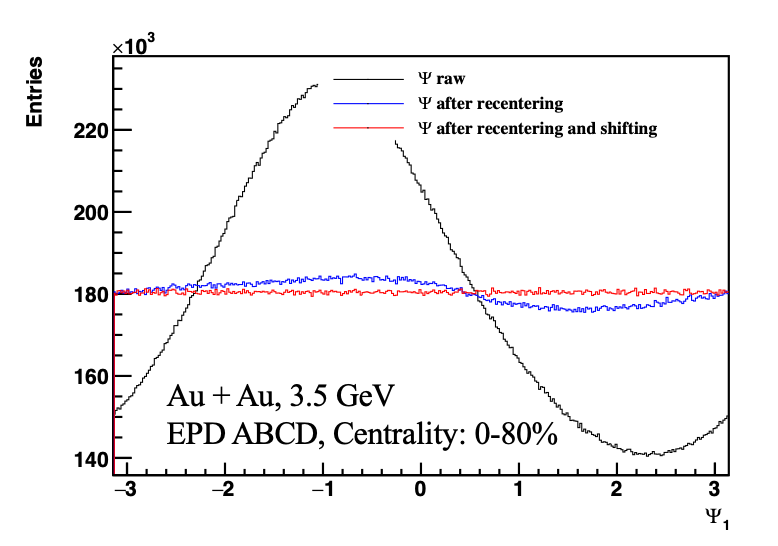
\includegraphics[width=0.45\linewidth]{figures/chapter02/EP_3p5GeV.png}
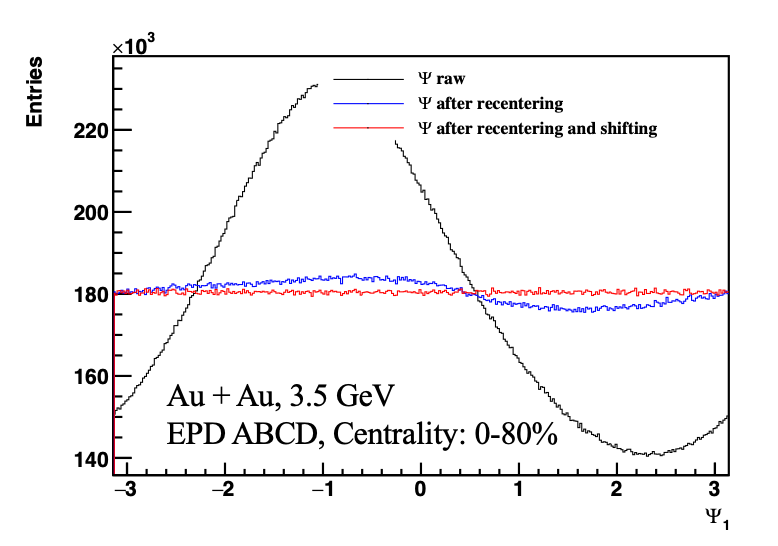
\includegraphics[width=0.45\linewidth]{figures/chapter02/EP_3p5GeV.png}
\caption{The event plane distribution on EPD.}
\label{fig:EP_distribution}
\end{figure}

\subsubsection{Event plane resolution}
After recentering and shifting calibration, the event plane is ready for the flow calculation. 
While the finite multiplicity in the experiment would limit the estimation of the reaction plane angle.~\cite{voloshin2008collective}
So the event plane resolution would be brought to correct the oberverd flow coefficients, which could be expressed as equation~\ref{eq:resolution}
\begin{equation}
R_n=\left\langle\cos \left[n\left(\Psi_n-\Psi_{\mathrm{r}}\right)\right]\right\rangle
\label{eq:resolution}
\end{equation}
Where $\Psi_r$ is reaction plane angle, $\Psi_n$ is the event plane angle.
The angle brackets denote averaging over many events. 

In the fixed target mode, one would not be able to get sub-events are equal, since the collision happens at 
the end of TPC. The resolution in different window are not equal, one need at least three windows to determine
the event plane resolution in each of them.~\cite{poskanzer1998methods} It could be expressed as
\begin{equation}
    \left\langle\cos \left(n\left(\Psi_m^a-\Psi_r\right)\right)\right\rangle=\sqrt{\frac{\left\langle\cos \left(n\left(\Psi_m^a-\Psi_m^b\right)\right)\right\rangle\left\langle\cos \left(n\left(\Psi_m^a-\Psi_m^c\right)\right)\right\rangle}{\left\langle\cos \left(n\left(\Psi_m^b-\Psi_m^c\right)\right)\right\rangle}}
\label{eq:threeSub_res}
\end{equation}
Where $\Psi_m^a$ is the target event plane angle,  $\Psi_m^b$ and  $\Psi_m^c$ are the reference event plane angle.

In this analysis, we foucus on directed flow($v_1$) and elliptic flow($v_2$) measurement, they are both bashed on 
first order event plane. so we substitue $m=1$ to the equation~\ref{eq:threeSub_res}. According to the STAR published 3 GeV paper~\cite{Abdallah_2022},
One can get the largest resolution if chosen the forward eta window(EPD group A and B). We follow the method and take EPD group A and B 
as our target event plane. Other windows from EPD and TPC would be chosen as reference windows. They are divided as shown by Fig.~\ref{fig:EPD_TPC_groups}
This figure is specical for 3.0 GeV. We note here eta could reach 2.4 for 3.2, 3.5 and 3.9 GeV data, since inner TPC was upgarded at these three energies, 
and eta gap in the TPC is $[-1.15, -1.25]$.
\begin{figure}[hbt!]
\centering
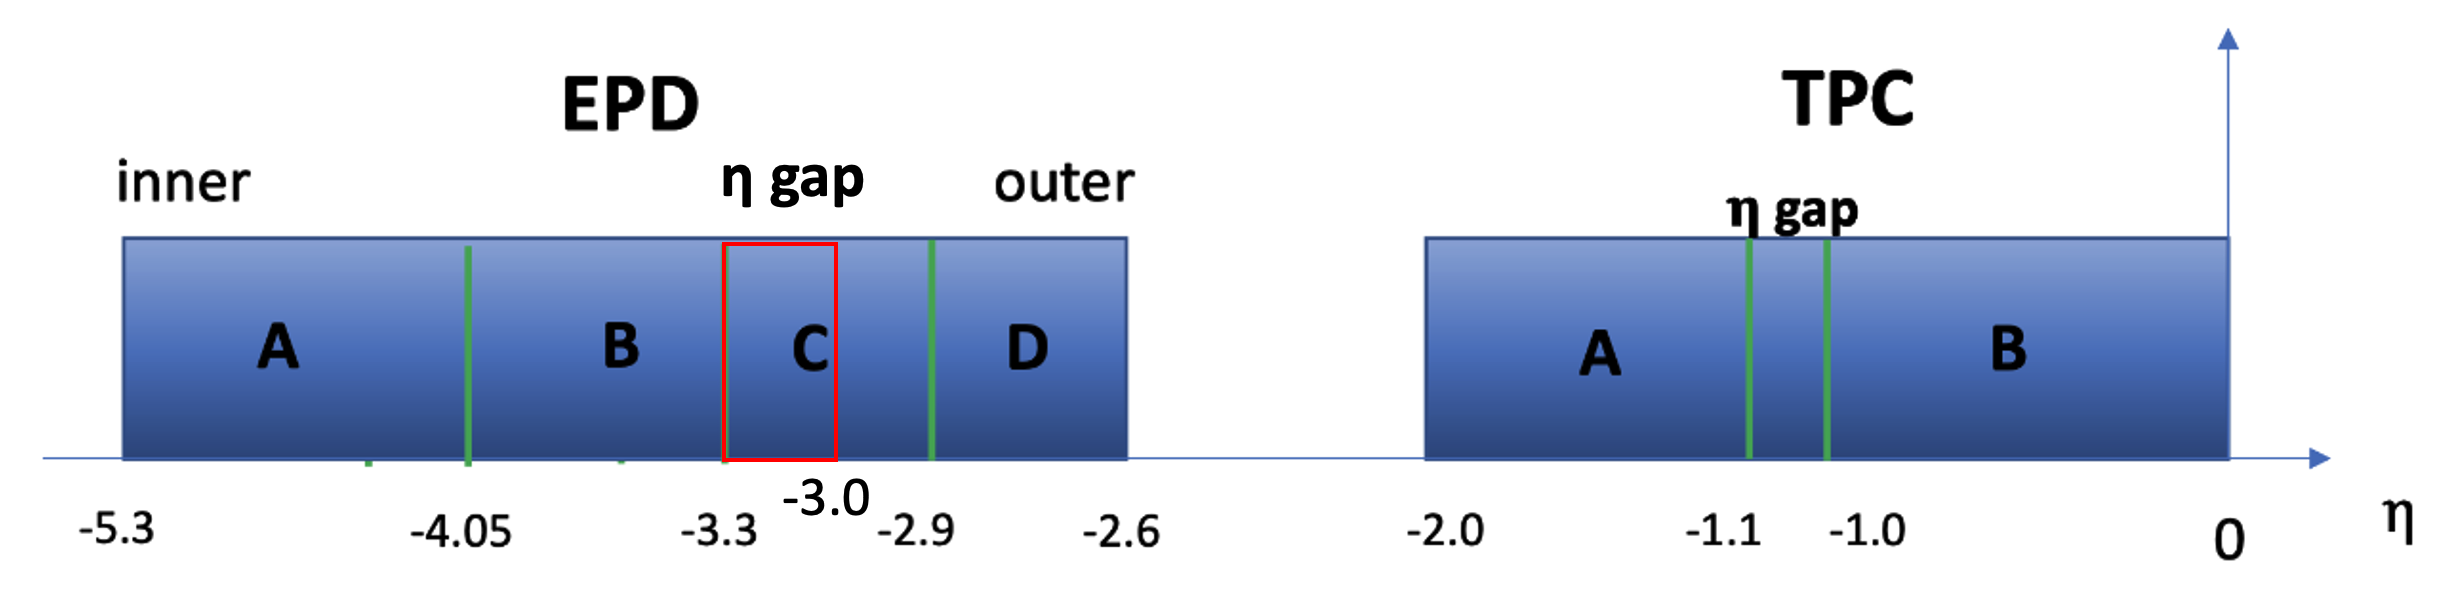
\includegraphics[width=0.65\linewidth]{figures/chapter02/EPD_TPC_groups.png}
\caption{The sketh of EPD and TPC groups.}
\label{fig:EPD_TPC_groups}
\end{figure}

%\begin{equation}
%v_n=\frac{v_n^{\mathrm{obs}}}{R_n}
%\label{eq:vn}
%\end{equation}


\subsection{Particle identification}



\subsection{Efficiency correction}
